% Első előadás - bevezetés

\chapter{Bevezetés}

\section{A tárgy célja}
A tárgy célja ismertetni a jelenleg domináns architektúrákat (Intel Core, AMD Zen, ARM), speciális témaköröket (pl. disszipáció) és a mobil architektúrákat.

\section{Csíkszélesség}
A processzor csíkszélessége a hagyományos (planár) MOSFET tranzisztorokat használó processzoroknál a tranzisztor kapu szélességét jelenti.
Az Intel által bevezetett 3D FinFET tranzisztorok jellemzéséhez már több paraméterre lenne szükség, de a publikációkban továbbra is egy számot használtak.
Ezért gyártónként eltérően kell értelmezni a gyártástechnológiát. Pl. az Intel 10 nm technológiája nagyjából a Samsung vagy a TSMC 7 nm-esének felel meg.

\section{Pentium 4 processzorcsalád}
A Core 2 család elődje a Pentium 4 processzorcsalád volt, ami valójában 3 generációt jelent (Willamette, Northwood, Prescott).
A Pentium 4 fontos innovációkat tartalmazott, alapja a Netburst mikroarchitektúra.
Második generációja hozta be először a többszálas architektúrát, a harmadik pedig a 64 bites architektúrát és a több processzormagot (Pentium D).

2000-ben 7 éves élettartamot vártak a Netburst-től, de 2004 körül a bejelentett architektúrákat visszavonták, mivel a várt 10 GHz-es frekvencia helyett csak 3.6-at értek el, a disszipáció miatt.
A Prescott processzorok 1 cm\textsuperscript{2}-en 100 W-ot adtak le, amivel elérte a léghűtéses rendszerek határát.

\section{Intel Core processzorok fejlesztése}
A fejlesztők ezentúl másik irányban folytatták a tervezést, a nyers teljesítmény növelése helyett az 1 W-ból kihozható teljesítmény maximalizálására törekedtek.
2006 környékén a mobil processzorok megjelenésével egy újabb tervezési irány jelent meg: a minél alacsonyabb fogyasztás, a jobb üzemidő elérése miatt.

A célok elérése érdekében a Pentium 4-ig használt egyfázisú fejlesztési modellt két fázisúra (Tick-Tock) cserélték.
Az első fázisban döntően a csíkszélesség csökkentésére fókuszáltak, a másodikban pedig a mikroarchitektúrát fejlesztették.
Ez a fejlesztési modell a Core 2 processzorcsaládtól kezdődött, és a Skylake-ig tartott, amit viszont nem követett csíkszélesség csökkentés, így a fejlesztés visszaállt egy fázisúra.

\section{Gyártási technológia}
A gyártástechnológia fejlődése a \ref{fig:nm}. ábrán látható.
Látható, hogy 22-14 nm környékén lelassult a fejlődés.
\begin{figure}[H]
    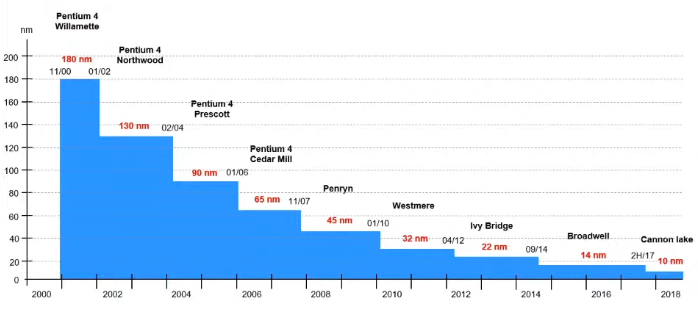
\includegraphics[width=\textwidth]{nm}
    \centering
    \caption{Intel processzorok csíkszélessége}
    \label{fig:nm}
\end{figure}

Az Intel ennek ellenére 2019-ben két évenkénti csíkszélesség csökkentést jósolt 2029-ig.

\section{Utasításkészlet fejlődése}
Az utasításkészlet legfontosabb fejlesztése a vektorfeldolgozás volt, először 64 biten, majd a későbbiekben 128, 256 és újabban 512 bitre szélesítették.

\section{A mikroarchitektúra fontosabb újításai}
A Core 2 processzorok 3 helyett 4 széles magokat használtak, kb. 30\%-al nagyobb teljesítményt eredményezve.
Ezzel lehagyta az AMD-t.
A Nehalem architektúránál jelent meg az integrált memóriavezérlő és a 3. szintű cache, valamint újra a többszálú végrehajtás.
A Sandy Bridge legfőbb újdonsága a lapkára integrált videokártya volt.
A Skylake 5 széles magokat alkalmazott és megjelentek az egy tokba integrált CPU, GPU és nagy teljesítményű memória lapkák.
2017-ben az AMD konkurenciájára válaszul az Intel növelte a magok számát 6-ra, 8-ra, majd 10-re.

Egy másik fontos fejlődési irány a disszipáció kezelése volt, erről később részletesebben.

\section{Fejlődés IPC-ben kifejezve}
Az ábrán látható, hogy az architekturális váltást hozó processzorok jóval nagyobb (kb. 10\%) teljesítmény növekedést hoztak, mint a technológiai váltást hozók.
\begin{figure}[H]
    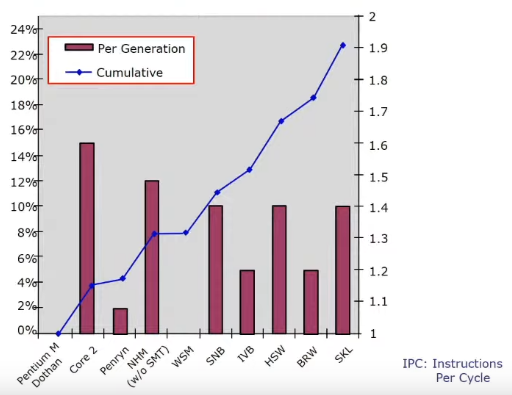
\includegraphics[width=\textwidth]{ipc}
    \centering
    \label{fig:ipc}
\end{figure}

\section{Frekvencia vs tranzisztorok száma}
A következő ábra jól mutatja, hogy az utóbbi kb. 20 évben megállt a frekvencia növekedése, a fejlődés fő iránya a tranzisztorok számának növelése és az energiahatékonyság.
\begin{figure}[H]
    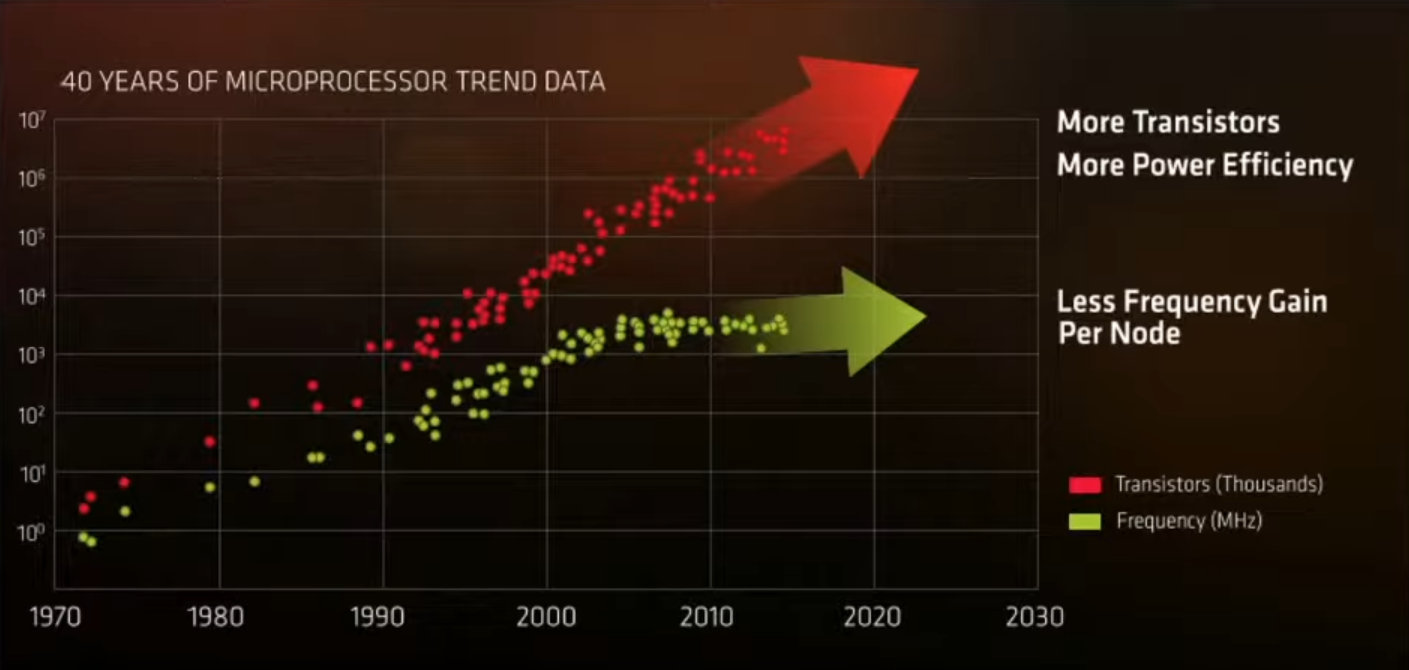
\includegraphics[width=\textwidth]{moore}
    \centering
    \label{fig:moore}
\end{figure}